\chapter{Solution prototype}\label{chap:chap3}


\section{The problem it solves}

As already described in Section \ref{sec:goals}, this dissertation aims to solve
the problem of PPLs having too much of a steep learning curve for someone who
is unexperienced in programming, even if that person would've enough knowledge
in statistics to leverage PPLs' power in applied machine learning. We propose
to do so by developing a visual programming environment for a PPL that is user-friendly
and yet flexible enough to be able to program solutions for non-trivial problems.

Since the existing work joining VP with PP is still nonexistent, the notable exception
being VIBES and WinBUGS (even if it has its shortcomings, as described in \ref{sec:vibes}),
we have identified margin for improvement.

VPEs have been successfuly
applied to other domains, and considering previous studies in VP that suggest it is
well suited for both limited domains and unexperienced programmers, it is the
author's belief that development in PPLs would also benefit from such a tool.
Therefore, we intend to validate the following hypotehsis:

\begin{quote}
  ``When a user instead of specifying a model textually,
  produces the model via a graphical representation that automatically translates
  itself into executable code, he will do so in a shorter amount of time, make
  fewer errors (both during development and regarding the final solution) and
  will reach a final representation that is more understandable and thus
  easier to maintain.''
\end{quote}

Because there isn't a standard method for evaluating if a language is easier
to work with than another, the question arises on how to evaluate success.
The optimal way to do so would be to make an empiral
study. However, this requires having a tool mature and stable enough so that the
study's results can be considered reliable and representative of an underlying
idea (in this case, that a VPE can boost user's performance when developing
models with a PPL). The goal of this dissertation is to
assess several ways how such a tool could be built, pick one of them and develop
a prototype; is is not to develop production-grade software.

An alternative to this empirical evaluation is to gather examples of probabilistic programs expressed in a
PPL (either the one who chose to serve as backend, or another with similar
capabilities) in its traditional textual form, translate them into our graphical
language, and compare the two forms. This what we will be doing.

\subsection{An empirical study}

The way the study would work would be by compare how fast an user can define a model for a given set of problems
when using a VPL in a regualr way or through our graphical interface. We'd then
count the number of syntax and type erros done with each representation. By
selecting users who never used the given PPL, we could not only measure execution
speed but learning time.

It would also be valuable to assess, not only how fast can someone develop with either
of the alternatives, but also the quality of the output. That could be done in two
steps: starting by verifying if the program correctly models the problem and then
asking the participants in the study if they believe the model they
have developed graphically is easier to understand than its textual counterpart (and
vice-versa).
Although subjetive, we believe getting the participants' opinion
regarding the output quality could provide valuable insights in order to understand if VP can
really enhance an user's experience when using a PPL. Another method we could use
to help us make an assessment of the validity of the hypothesis would be asking
participants questions regarding usability. Even if it may seem redundant, since
we would already have the time measurements, it is a way of identifying strenghts and
weaknesses with reduced granularity.

\subsection{Target audience}

The resulting tool is aimed at people with knowledge in statistics
who are unexperienced programmers. This may include data scientists, researchers,
mathematicians or staticians. In short, anyone who would apply PP to problem
solving but are not fluent in programming.

\subsection{Expected contributions}

By the end of this work, we would expect to have built a VPE for PPLs that can
be extended with more PPLs, even if we are only implementing the adapter for one.
By doing so we will: have a platform that enables other people to experiment
and make usability research on, define a visual language that can be applied to PP in general,
identifying what works and what to avoid,
and ultimately assessing the viability of applying VP to PP to enhance end-user's
productivity.

\section{Outline}

As we have seen in Chapters \ref{chap:intro} and \ref{chap:sota}, there is a
rising awareness of the power of ML methods. PPLs, despite still being mostly
unknown to data scientists, provide an interface for defining personalized
probabilistic models and possess a built-in inference engine.
The benefits of VPLs when compared to a textual format are well-known, but there
is no VPL applied to a PPL, so we aim to create one.

A big requirement we wished to fulfill was, not only ease of use, but also ease
of installation. This means having portability across operating systems as well
as being able to execute without installing dependencies. For this reason, we
decided our VPE should run in the browser.

It was also important that we chose
a target PPL for which there is a decent amount of programs written on it, so we
could thoroughly test our hypothesis. Because it was the one
that best matched this criteria we chose Infer.NET to work with, a framework that
can be used in CLI languages (such as C#, F# or C++). Because none of these
languages can, at least at the time of writing (that might change when WebAssembly
\cite{weba} gets widespread support), be directly compiled to JavaScript
we will be sacrificing immediate
visual feedback and build a hybrid text and visual system (a VPE) rather than a purely
visual language (see Section \ref{sec:vpe} for more details). This means that
our tool won't be able to run the model the user defines, but will generate
Infer.NET (hosted in C#) code (see Figure \ref{fig:scope}).

The user can take the generated
code and run it in a separate runtime (such as CLR). While not the ideal scenario, because it
complicates the development and debugging cycles (in order to see each change,
users must first copy the code to a file in a machine that can compile and run it),
it has the advantage of seamlessly integrating with larger projects. An example
would be an enterprise application written in C# that has a small component
that the team who's developing it feels it would make sense to use a PPL there.
They can use our VPE to develop that portion of the program, and then just place
the code in the desired place. Using a purely visual programming language in the
same scenario, despite having a faster development time, would then require
a rewriting in a textual form.

\begin{figure}[t]
  \begin{center}
    \leavevmode
    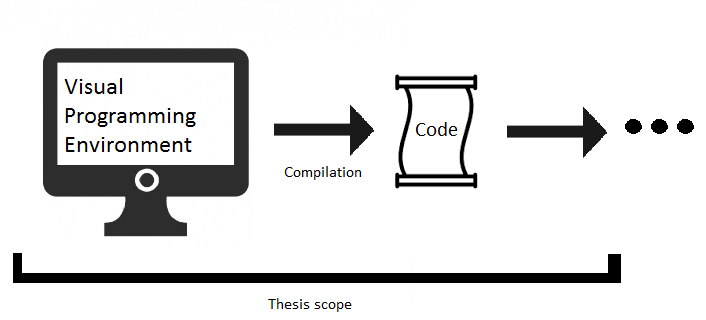
\includegraphics[width=0.86\textwidth]{scope}
    \caption{High-level look into our tool}}
    \label{fig:scope}
  \end{center}
\end{figure}

\section{Architecture}

\section{Implementation}

 % "controlled dataflow vpl"
 In this section we will be explaining why we made certain choices, such as for
 the target PPL, the front-end framework or what features to include or not.

\subsection{Picking a target PPL}

Perhaps one of the most important decisions we had to made concerns the PPL we
would be offering a VPE to, since the visual programming concepts applied are
highly dependent on the language's own capabilities. For instances, we cannot
study how VP can be helpful in an object-oriented design if we are using a
purely functional PPL such as Church which does no have that concept.

As we seen on Section \ref{sec:ppls}, the PPL landscape is heterogeneous enough
that we could pick a language from any paradigm or runtime we wanted to, as there
are many alternatives available. So we could narrow down the scope, we decided to avoid
purely functional and logical programming languages, because we wanted to build
a VPE that was not an end in itself: meaning that it was not only useful to build
PP but also to help our target audience eventually transition from a graphical
environment to the textual form (or, at least, be able to use both if they need
a more fine-grained control in a certain scenario). Even if it is a matter of
debate which paradigm is more suitable to people learning how to program, we feel
that because imperative and object-oriented are more common in data science (the prime
examples being Python and R), they would be a better choice.

After applying this restriction, there were still many PPLs to chose from, so
we decided upon the main criteria on which to make our decision: the language
should have comprehensible and extensive documentation, plenty of code examples
with a variety of complexities, an active and helpful community, be hosted in
a mainstream programming language (as opposed to being a standalone language by itself)
and it should run on the browser. The first three points are related to how well
can we learn the language well enough to design a VPE for it, having no prior
experience with it, in a short amount of time. Being executable on the browser
would allow to provide instant visual feedback of the results, since the VPE
would not be limited to defining a model, but it would could execute it.

On a technical side the strongest candidate is VentureScript \cite{probcomp},
due to the fact it is hosted in javascript (with the aforementioned advantages).
Despite this advantage, it is still on Alpha and both the code examples and
documentation are still scarce, even taking into consideration its predecessor's
examples \cite{forestdb} and tutorials \cite{church}.

The three stronger candidates, after some selection, were PyMC \cite{pymc},
Figaro \cite{figaro} and Infer.NET \cite{InferNET14}. All three are hosted in popular languages
(Python, Scala and C#/F#, respectively) and have comprehensive tutorials and
documentation available \cite{pymct}\cite{figarot}\cite{InferNET14t}.

We ended up choosing Infer.NET because it had the widest range of examples
available, which is pivotal to design a VPE as complete as possible, as well
as evaluate it under different scenarios. Besides its complete documentation
and tutorial, its website features more than 20 code examples, as well as a list
of papers that resorted to Infer.NET. Some of these papers are about PP or PPL theory,
but others are about applications of it, such as "Automatic analysis and
identification of verbal aggression and abusive behaviors for online social
games" \cite{balci2015automatic}, which gives us confidence that Infer.NET is
mature enough so we can focus in the VPE design rather than struggling with
learning the language. Bottom line, it was chosen due to the abundant number of
programs written on it publicly available.

\subsection{Picking a front-end}

\subsubsection{Blockly}

\subsubsection{GoJS}

\subsubsection{Custom implementation}

\subsection{Defining a Grammar}

\subsection{Handling Cycles and Conditionals}

\subsection{Handling objects and arrays}

\subsection{Inverse Compilation}

\subsection{Instant visual results}

\subsection{Opening to extension}

\section{Tutorial}

\section{Conclusions}
